\section{Simulation} \label{sec: Simulation}
Describes the result of the behavioral simulation based on the synthesized hardware description language.

\subsection{Part I: behavioral simulation of decoder} \label{subsec: Part I: behavioral simulation of decoder}
After a successful simulation of the synthesized hardware description language that implements an decoder a test bench was written, see listening \ref{lst: Testbanche decoder}. The time variant simulation is shown in figure \ref{fig: Vivado_lab1_BS} which shows steps trough the different possible switch positions and shows the output on the decoder bus seg. In comparison to the simulation given in Lab 02 Part 1 it could be confirmed that there are mostly identical.

\begin{figure}[ht]
	\centering
	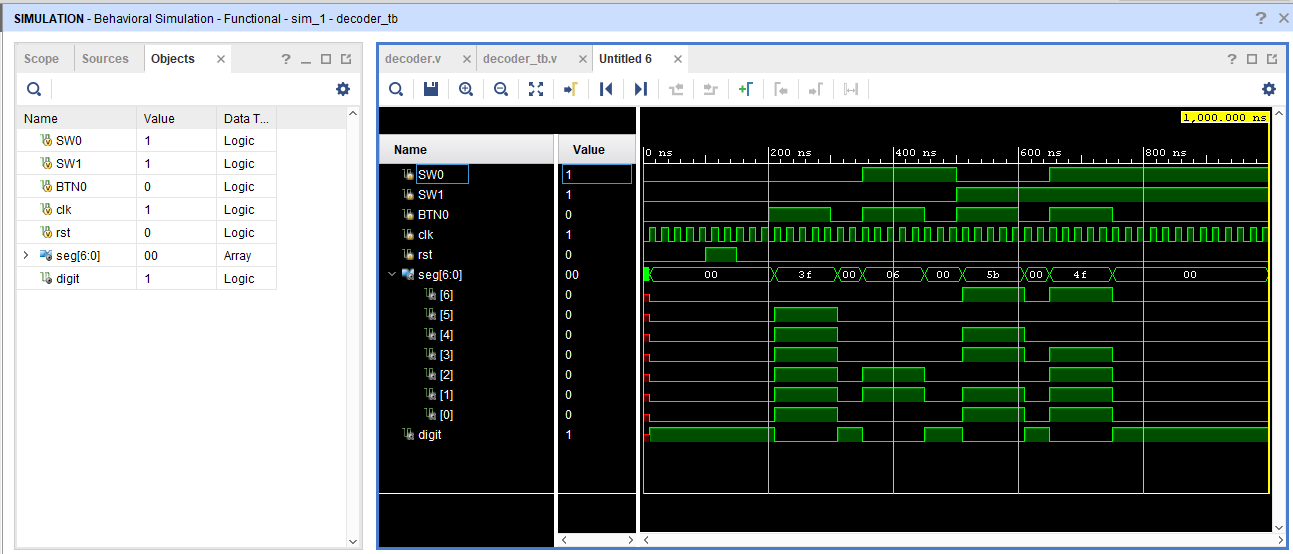
\includegraphics[width=1.0\textwidth ]{01_images/Vivado_lab1_BS.PNG}
	\caption{Vivado behavioral simulation of the decoder module.}
	\label{fig: Vivado_lab1_BS}
\end{figure}


%\subsection{Virtual Machine VM}\label{subsec: Virtual Machine}
%A virtual machine is used to run Ubuntu 18.04 LTS which is supported for five years and is free of charge. The reason to do so is that software can be developed in an environment while then at the end of the project the entire environment can be shipped and not only code. The software used is VMware Player 14.
%
%\begin{description}
%	\item[VM name] RAMI\_RF\_TUNER
%	\item[username] rami
%	\item[password] 1234
%\end{description}
%
%\subsection{Software Tools}\label{subsec: software_tools}
%Used for documentation is 
%\begin{enumerate}[(a)]%for capital roman numbers.
%	\item Git, GitHub
%	\item \LaTeX
%	\item MiK\TeX Consol
%	\item \TeX Studio
%	\item Pandoc \linebreak
%	is used for Markdown to Latex conversion
%	\item Altium Designer v15.1
%\end{enumerate}
%
%\subsection{Git, GitHub}\label{subsec: install_git}
%\href{https://git-scm.com/downloads}{Git} is a fast-version-control tool that  allows the engineer to jump back to any commit that he made. It is available on the three major operating systems Windows, Mac OS X, and Linux/Unix. For Windows there is an additional benefit git comes with a built in Linux/Unix bash terminal so that Linux/Unix commands can be used on Windows and is called Git Bash.
%
%Install Git on Ubuntu 18.04 LTS
%Open the terminal and type Git. If Git is not installed it will show as listing \ref{lst:git install on ubuntu}. Just in case you haven't been working yet with Linux the password is never shown by typing it. After a successful installation the version can be checked.
%\begin{lstlisting}[language=bash,caption={git common commands},label=lst:git install on ubuntu]
%rami@ubuntu:~$ git
%Command 'git' not found, but can be installed with:
%sudo apt install git
%
%rami@ubuntu:~$ sudo apt install git
%[sudo] password for rami: 
%
%rami@ubuntu:~$ git --version
%git version 2.17.1
%
%\end{lstlisting}
%
%Initializing a git repository in an existing folder locale:
%\begin{lstlisting}[language=bash,caption={Initializing a git repository},label=lst: git init]
%    $ git init
%    $ git add README.md
%    $ git commit -m "first commit"
%    $ git remote add origin https://github.com/userName/repositoryName.git
%    $ git push -u origin master
%\end{lstlisting}
%...or cloning an existing repository from GitHub a git repository in an existing folder locale:
%\begin{lstlisting}[language=bash,caption={Clone git repository},label=lst: git clone]
%    $ git clone https://github.com/userName/repositoryName.git
%\end{lstlisting}
%…or push an existing repository from the command line
%\begin{lstlisting}[language=bash,caption={Remote git repository on GitHub},label=lst: git remote]
%    $ git remote add origin https://github.com/haringd/GeocalculatoriOSHW7.git
%    $ git push -u origin master
%\end{lstlisting}
%…or most common git commands used in the command line
%\begin{lstlisting}[language=bash,caption={git common commands},label=lst:git common]
%    $ git pull
%    $ git status
%    $ git add .
%    $ git commit -m "Your commit text"
%    $ git push
%    
%    $ git log
%    $ git checkout <commit>
%\end{lstlisting}
%
%
%
%
%\subsection{Install \LaTeX}\label{subsec: install_latex}
%\subsubsection{Install MiKTeX}\label{subsubsec: install_miktex}
%\href{https://miktex.org/}{MiKTeX} provides package management for \LaTeX that handles most packages used for documentation.  
%
%\subsubsection{Install TexStudio}\label{subsubsec: install_texstudio}
%\href{https://www.texstudio.org/}{TexStudio} is a convenient front end to edit and write \LaTeX syntax. Like most IDEs it provides auto-completion (ctrl + space). It also provides compiler and build system to convert \LaTeX into a PDF format. Furthermore it integrates easy into git which makes it easier to collaborate in a team.
%
%\subsection{TexStudio Hints}\label{subsec: texstudio_hints}
%\subsubsection{Edit Default Language and Dictionary}
%As shown in Figure \ref{fig: texstudio_selectDefaultLanguage}, this can be done under Preferences -> Language Checking.
%
%
%\subsubsection{Convert a *.md file into a *.tex file}
%Pandoc can be used to convert, with a simple terminal command, a *.md file into a *.tex file. Easiest is to convert the file as pre compiler option which can be added shown in Figure \ref{fig: texstudio_convertMDfiletoTEXfilewithPandoc}. The terminal command is shown in Listing \ref{lst: pandoc_bash_convert_file}
%
%\begin{lstlisting}[language=bash, caption=Terminal command that converts .md to .tex files, label=lst: pandoc_bash_convert_file]
%pandoc -f markdown -t latex -o onepage.tex ONEPAGE.md.
%\end{lstlisting}
%
%\begin{figure}[ht]
%	\centering
%	\includegraphics[width=400px ]{01_images/texstudio_convertMDfiletoTEXfilewithPandoc}
%	\caption{Language Settings in TexStudio.}
%	\label{fig: texstudio_convertMDfiletoTEXfilewithPandoc}
%\end{figure}
%
%\subsection{biblatex, make citations with \LaTeX}\label{subsec: Bibtex, make citations with LaTeX}
%In order to run the citation properly use the following commands in bash or windows terminal on the file.
%\begin{verbatim}
%    $ pdflatex reportRFTuner
%    $ biber reportRFTuner
%    $ pdflatex reportRFTuner
%\end{verbatim}
%That solves the problem of not showing the citations after editing the *.bib file correctly.
%
%An easy way to handle citations is to use \href{https://www.mendeley.com}{Mendeley} which allows to copy a citation in bibtex format and simply append it to the *.bib file. Just in case you wonder where you got bibtex from it was installed with miktex or texstudio. 
%
%A bibtex file *.bib has the following syntax and is used with the \\cite{Vizmuller1995} command:
%
%\begin{lstlisting}
%	@book{Vizmuller1995,
%		address = {Boston, London},
%		author = {Vizmuller, Peter},
%		isbn = {0-89006-754-6},
%		mendeley-groups = {RF{\_}TUNER RAMI{\_}2018},
%		pages = {281},
%		publisher = {Artech House, Inc.},
%		title = {{RF Design Guide}},
%		year = {1995}
%	}
%	@misc{key_to_cite_a_webpage_as_example,
%	mendeley-groups = {RF{\_}TUNER RAMI{\_}2018},
%	title = {{Multi-Aperture cores (2867000102) - Fair Rite}},
%	url = {https://www.fair-rite.com/product/multi-aperture-cores-2867000102/},
%	urldate = {2018-07-18}
%	}
%	
%\end{lstlisting}
%
%\subsection{Altium Designer v15.1}\label{subsec: Altium Designer v15.1}
%This is an Altium Designer, short Altium, tutorial that shall guide the user trough the most common steps of Altium.
%
%It is assumed that Altium  is installed on your PC or you have access to it trough the GVSU software of the School of Engineering. 
%
%\begin{enumerate}
%	\item
%Pres Windows key on keyboard and type "Altium" and press enter or double click on Altium Icon, see figure \ref{fig: Altium Icon} on your Desktop if available to start the software package.
%
%\begin{figure}[htbp]
%	\centering
%	\includegraphics[width=0.3\textwidth]{01_images/Altium_Icon.PNG}
%	\caption{Altium Icon.}
%	\label{fig: Altium Icon}
%\end{figure}
%
%\item 
%Altium starts and if no project is open it should look like figure \ref{fig: Altium No Project open}.
%\begin{figure}[H]
%	\centering
%	\includegraphics[width=0.7\textwidth]{01_images/Altium_noProject.PNG}
%	\caption{Altium No Project open.}
%	\label{fig: Altium No Project open}
%\end{figure}
%
%\item
%To start a new project select in menu bar "File" $\rightarrow$ "New" $\rightarrow$ "Project" as shown in figure \ref{fig: Altium new Project}.
%\begin{figure}[H]
%	\centering
%	\includegraphics[width=0.7\textwidth]{01_images/Altium_newProject.PNG}
%	\caption{Altium new Project.}
%	\label{fig: Altium new Project}
%\end{figure}
%
%\item
%The Altium new project dialog appears. Select "PCB Project" in the first column and default in the second one. 
%In the field Name you chose an appropriate project name like "Test1" as example.
%In the field Location you chose an appropriate space to store the project. On your own machine it is beneficial if it is somewhere on the C: drive or on an GVSU blade server on the W: drive. 
%The version control is unchecked as well as the Managed Project.
%If version control is desired the best why to do it, according the authors personal opinion, is to create the project into a git repository and do the version control manually with git in combination with GitHub or GitLab.  \\
%\textbf{Note:} In the naming and location instead of spaces use underscores this avoids unwanted magic errors.   
%\begin{figure}[H]
%	\centering
%	\includegraphics[width=0.7\textwidth]{01_images/Altium_newProjectDialog.PNG}
%	\caption{Altium new Project dialog.}
%	\label{fig: Altium new Project dialog}
%\end{figure}
%
%\item
%The Altium generated now an empty project which appears in the Project view bar on the left side as shown in figure \ref{fig: Altium empty Project}. The project does not contain any documents yet.
%\begin{figure}[H]
%	\centering
%	\includegraphics[width=0.7\textwidth]{01_images/Altium_emptyProject.PNG}
%	\caption{Altium empty Project.}
%	\label{fig: Altium empty Project}
%\end{figure}
%
%\item
%The first thing is to add a schematic sheet which allows to draw a circuit. To add a schematic right click on the empty project $\rightarrow$ Add New to Project $\rightarrow$ Schematic. It is possible to do the same step in menu bar "File" $\rightarrow$ New... $\rightarrow$ Schematic. If the second procedure is used be aware that if you have multiple projects the new schematic sheet will be added to the selected project in project view window.
%\begin{figure}[H]
%	\centering
%	\includegraphics[width=0.7\textwidth]{01_images/Altium_addSchematic.PNG}
%	\caption{Altium add Schematic sheet.}
%	\label{fig: Altium add Schematic}
%\end{figure}
%
%\item
%After a document is generated it is good practice to save it. Chose a expressive name for the sheet, and keep in mind that Altium allows you to build an hierarchical sheet structure with top level and multiple sheets. Furthermore, Altium is a huge software package which results in complexity, so it can crash a lot, save often! The short cut to save is \textbf{CTRL+S}  
%\begin{figure}[H]
%	\centering
%	\includegraphics[width=0.7\textwidth]{01_images/Altium_saveScheet.PNG}
%	\caption{Altium save schematic sheet with an expressive name.}
%	\label{fig: Altium_saveSheet }
%\end{figure}
%
%\item
%In the generated document which is a schematic sheet the Document options have to be set. Right click mostly anywhere on the schematic sheet and  
%\begin{figure}[H]
%	\centering
%	\includegraphics[width=0.7\textwidth]{01_images/Altium_DocumentOptions.PNG}
%	\caption{Altium change options of the generated Document in this case a schematic sheet.}
%	\label{fig: Altium_DocumentOptions }
%\end{figure}
%
%
%\end{enumerate} %ALtium designer
%
%\begin{table}[ht]
%	\begin{center}
%		\begin{tabular}{|| c | c  ||} 
%			\hline
%			Shortcut & Description  \\ 
%			[0.5ex] 
%			\hline\hline
%		
%			\textbf{CTRL+S} & Save selected document \\ \hline
%			\textbf{p} & Press "P" as your mouse is over an open document to open placement options. \\ \hline

%		\end{tabular}
%	\end{center}
%	\caption{$\mu C$ pin occupation}
%\end{table}
